
\begin{frame}{对数的定义}
    \begin{block}{定义}
        若 $a > 0$,$a \neq 1$,且 $a^y = x$,则称 $y$ 是以 $a$ 为底 $x$ 的对数,记作:
        \[
        y = \log_a x
        \]
        其中,$a$ 称为底数,$x$ 称为真数,且 $x > 0$。
    \end{block}
    
    \begin{alertblock}{指数与对数的关系}
        \[
        a^y = x \iff y = \log_a x (\text{指数式和对数式互换})
        \]
    \end{alertblock}
    
    \begin{exampleblock}{特殊对数}
        \begin{itemize}
            \item 自然对数:$\ln x = \log_e x$($e \approx 2.71828$)
            \item 常用对数:$\log x = \log_{10} x$
        \end{itemize}
    \end{exampleblock}
  \end{frame}
  
  \begin{frame}{对数运算法则}
    \begin{block}{基本运算法则}
        设 $a > 0$,$a \neq 1$,$M > 0$,$N > 0$,则:
        \begin{enumerate}
            \item $\log_a(MN) = \log_a M + \log_a N$
            \item $\log_a\left(\frac{M}{N}\right) = \log_a M - \log_a N$
            \item $\log_a(M^n) = n \log_a M$($n \in \mathbb{R}$)
        \end{enumerate}
    \end{block}
    
    \begin{alertblock}{注意事项}
        \begin{itemize}
            \item 真数必须大于零
            \item 底数$a$必须满足 $a > 0$ 且 $a \neq 1$
            \item 运算法则只适用于同底数的对数
        \end{itemize}
    \end{alertblock}
    \begin{block}{对数恒等式}
      \begin{itemize}
        \item     $\log_a a^N =N \quad (a > 0, \, a \neq 1)$
        \item     \(a^{\log_a N} = N \quad (a > 0, \, a \neq 1, \, N > 0)\)
    \end{itemize}
  
  \end{block}
  
  \end{frame}
  
  
  
  
  \begin{frame}{换底公式}
    \begin{block}{换底公式}
        对于任意 $a > 0$,$a \neq 1$,$b > 0$,$b \neq 1$,$x > 0$,有:
        \[
        \log_a x = \frac{\log_b x}{\log_b a}
        \]
    \end{block}
    
    \begin{alertblock}{推论}
        \begin{enumerate}
            \item $\log_a b = \frac{1}{\log_b a}$
            \item $\log_{a^n} b = \frac{1}{n} \log_a b$
            \item $\log_a b \cdot \log_b c = \log_a c$
        \end{enumerate}
    \end{alertblock}
    
    \begin{exampleblock}{应用场景}
        \begin{itemize}
            \item 计算对数的值(如 $\log_2 5 = \frac{\ln 5}{\ln 2}$)
            \item 化简对数表达式 .
        \end{itemize}
    \end{exampleblock}
  \end{frame}
  
  
  
  
  \begin{frame}{对数函数的图像与性质}
    \begin{columns}
        \begin{column}{0.5\textwidth}
            \begin{block}{当 $a > 1$ 时}
                \begin{itemize}
                    \item 定义域:$(0, +\infty)$
                    \item 值域:$(-\infty, +\infty)$
                    \item 过定点 $(1, 0)$
                    \item 在 $(0, +\infty)$ 上单调递增
                \end{itemize}
            \end{block}
        \end{column}
        \begin{column}{0.5\textwidth}
            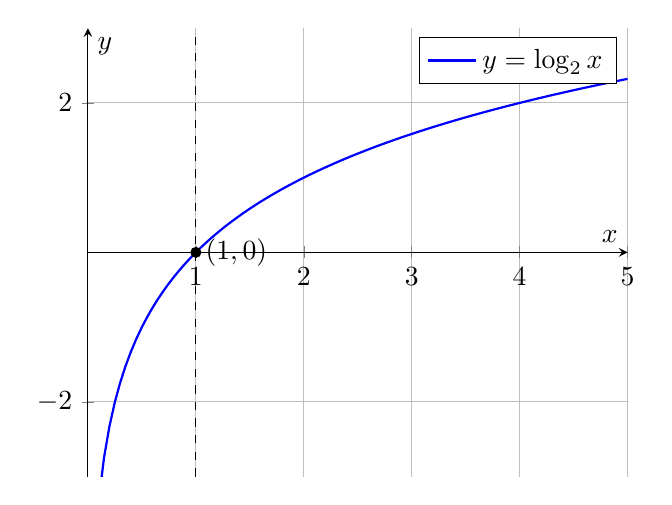
\begin{tikzpicture}
                \begin{axis}[
                    xmin=0, xmax=5,
                    ymin=-3, ymax=3,
                    axis lines=middle,
                    xlabel=$x$, ylabel=$y$,
                    grid=both,
                    samples=100,
                    domain=0.1:5
                ]
                \addplot[blue, thick] {ln(x)/ln(2)};
                \addlegendentry{$y=\log_2 x$};
                \draw[dashed] (1,-3) -- (1,3);
                \fill[black] (1,0) circle (2pt);
                \node[right] at (1,0) {$(1,0)$};
                \end{axis}
            \end{tikzpicture}
        \end{column}
    \end{columns}
  \end{frame}
  
  
  
  
  
  
  
  
  
  
  
  
  
  
  \begin{frame}{对数函数的图像与性质}
    \begin{columns}
        \begin{column}{0.5\textwidth}
            \begin{block}{当 $0 < a < 1$ 时}
                \begin{itemize}
                    \item 定义域:$(0, +\infty)$
                    \item 值域:$(-\infty, +\infty)$
                    \item 过定点 $(1, 0)$
                    \item 在 $(0, +\infty)$ 上单调递减
                \end{itemize}
            \end{block}
        \end{column}
        \begin{column}{0.5\textwidth}
            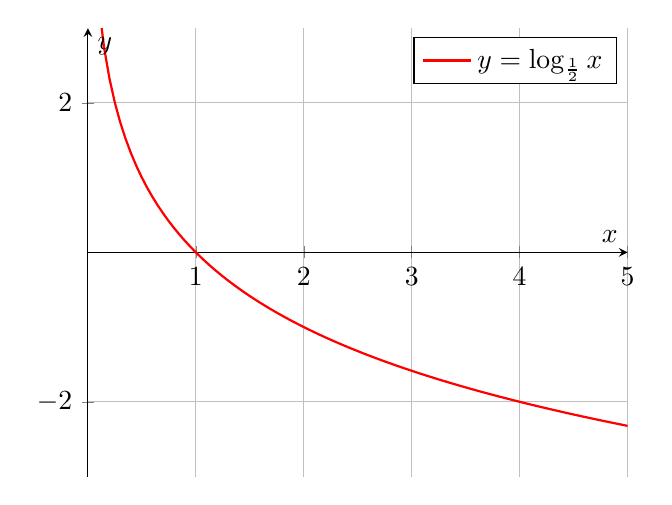
\begin{tikzpicture}
                \begin{axis}[
                    xmin=0, xmax=5,
                    ymin=-3, ymax=3,
                    axis lines=middle,
                    xlabel=$x$, ylabel=$y$,
                    grid=both,
                    samples=100,
                    domain=0.1:5
                ]
                \addplot[red, thick] {ln(x)/ln(0.5)};
                \addlegendentry{$y=\log_{\frac{1}{2}} x$};
                % \draw[dashed] (1,-3) -- (1,3);
                % \fill[black] (1,0) circle (2pt);
                % \node at (0,0) {$(1,0)$};
                \end{axis}
            \end{tikzpicture}
        \end{column}
    \end{columns}
  \end{frame}
  
  
  \begin{frame}{题目1:对数运算化简}
    \begin{block}{题目}
        化简下列表达式:
        \begin{enumerate}
            \item $\log_2 16 + \log_3 27$
            \item $\log_5 125 - \log_5 5$
            \item $\log_2 \sqrt{8} + \log_3 \frac{1}{9}$
        \end{enumerate}
    \end{block}
    
    \pause
    
    \begin{block}{答案}
        \begin{enumerate}
            \item $\log_2 16 + \log_3 27 = 4 + 3 = 7$
            \item $\log_5 125 - \log_5 5 = 3 - 1 = 2$
            \item $\log_2 \sqrt{8} + \log_3 \frac{1}{9} = \frac{3}{2} - 2 = -\frac{1}{2}$
        \end{enumerate}
    \end{block}
  \end{frame}
  
  
  
  \begin{frame}{题目2:对数方程求解}
    \begin{block}{题目}
        解下列方程:
        \begin{enumerate}
            \item $\log_3 x = 2$
            \item $\log_x 16 = 2$
            \item $\log_2 (x + 1) = 3$
        \end{enumerate}
    \end{block}
    
    \pause
    
    \begin{block}{答案}
        \begin{enumerate}
            \item $\log_3 x = 2 \implies x = 3^2 = 9$
            \item $\log_x 16 = 2 \implies x^2 = 16 \implies x = 4$($x > 0$且$x \neq 1$)
            \item $\log_2 (x + 1) = 3 \implies x + 1 = 2^3 \implies x = 7$
        \end{enumerate}
    \end{block}
  \end{frame}
  
  
  
  \begin{frame}{题目3:对数不等式求解}
    \begin{block}{题目}
        解不等式:
        \[
        \log_2 (x - 1) < 2
        \]
    \end{block}
    
    \pause
    
    \begin{block}{答案}
        \begin{enumerate}
            \item 定义域:$x - 1 > 0 \implies x > 1$
            \item 原不等式等价于:$\log_2 (x - 1) < \log_2 4$
            \item 由于底数 $2 > 1$,函数单调递增,故:
                  \[
                  x - 1 < 4 \implies x < 5
                  \]
            \item 结合定义域,解集为:$(1, 5)$
        \end{enumerate}
    \end{block}
  \end{frame}
  
  
  
  \begin{frame}{题目4:对数换底公式应用}
    \begin{block}{题目}
        计算:
        \[
        \log_2 3 \cdot \log_3 4 \cdot \log_4 5 \cdot \log_5 6 \cdot \log_6 7 \cdot \log_7 8
        \]
    \end{block}
    
    \pause
    
    \begin{block}{答案}
        \begin{enumerate}
            \item 利用换底公式:$\log_a b = \frac{\ln b}{\ln a}$
            \item 原式 $= \frac{\ln 3}{\ln 2} \cdot \frac{\ln 4}{\ln 3} \cdot \frac{\ln 5}{\ln 4} \cdot \frac{\ln 6}{\ln 5} \cdot \frac{\ln 7}{\ln 6} \cdot \frac{\ln 8}{\ln 7}$
            \item 约分后得:$\frac{\ln 8}{\ln 2} = \frac{3\ln 2}{\ln 2} = 3$
        \end{enumerate}
    \end{block}
  \end{frame}
  
  
  \begin{frame}{题目5:对数函数定义域与值域}
    \begin{block}{题目}
        求函数 $f(x) = \log_2 (x^2 - 4x + 3)$ 的定义域和值域。
    \end{block}
    
    \pause
    
    \begin{block}{答案}
        \begin{enumerate}
            \item 定义域:$x^2 - 4x + 3 > 0$
                  \[
                  (x - 1)(x - 3) > 0 \implies x < 1 \text{ 或 } x > 3
                  \]
            \item 令 $t = x^2 - 4x + 3$,则 $t$ 的取值范围为 $(0, +\infty)$
            \item 函数 $y = \log_2 t$ 的值域为 $(-\infty, +\infty)$
        \end{enumerate}
    \end{block}
  \end{frame}
  
  \begin{frame}[allowframebreaks]{题目6:对数函数定义域}
    \begin{block}{题目}
        求下列函数的定义域:
        \begin{enumerate}
            \item $f(x) = \log_3(2x - 5)$
            \item $g(x) = \ln(4 - x^2)$
            \item $h(x) = \log_{\frac{1}{2}}(x^2 - 2x - 3)$
            \item $k(x) = \frac{1}{\log_2(x - 1)}$
        \end{enumerate}
    \end{block}
    
    \pause
    
    \begin{block}{答案}
        \begin{enumerate}
            \item $2x - 5 > 0 \implies x > \frac{5}{2}$,定义域为$\left(\frac{5}{2}, +\infty\right)$
            \item $4 - x^2 > 0 \implies -2 < x < 2$,定义域为$(-2, 2)$
            \item $x^2 - 2x - 3 > 0 \implies (x - 3)(x + 1) > 0 \implies x < -1 \text{ 或 } x > 3$,定义域为$(-\infty, -1) \cup (3, +\infty)$
            \item $\begin{cases} x - 1 > 0 \\ \log_2(x - 1) \neq 0 \end{cases} \implies \begin{cases} x > 1 \\ x - 1 \neq 1 \end{cases} \implies x > 1 \text{ 且 } x \neq 2$,定义域为$(1, 2) \cup (2, +\infty)$
        \end{enumerate}
    \end{block}
  \end{frame}
  